\chapter{Geometría sintética}
\section{Planos afines sintéticos}
\begin{definition}[Plano afín]
Un \textbf{plano afín} es un par $\displaystyle \left(\mathcal{P}, \mathcal{R}\right) $ donde $\displaystyle \mathcal{P} $ es un conjunto no vacío cuyos elementos llamamos \textbf{puntos}, y $\displaystyle \mathcal{R} $ es un conjunto de subconjuntos de $\displaystyle \mathcal{P} $ cuyos elementos llamamos \textbf{rectas}, que satisfacen lo siguiente:
\begin{description}
\item[A1.] Sean $\displaystyle P,Q \in \mathcal{P} $ con $\displaystyle P \neq Q $. Existe una única recta $\displaystyle l \in \mathcal{R} $ tal que $\displaystyle P,Q \in l $ (escribimos $\displaystyle l = l\left(PQ\right) $).
\item[A2.] $\displaystyle \forall l \in \mathcal{R}, \forall P \in \mathcal{P} $, $\displaystyle P \not\in l $, existe una única recta $\displaystyle m \in \mathcal{R} $ tal que $\displaystyle P \in m $ y $\displaystyle m \cap l = \emptyset $.
\item[A3.] Toda recta tiene al menos dos puntos y hay al menos dos rectas.
\end{description}
\end{definition}
\begin{observation}
El tercer axioma asegura que se trata de algo dimensional.
\end{observation}
\begin{definition}[Rectas paralelas]
Si $\displaystyle l, m \in \mathcal{R} $ tales que $\displaystyle l \cap m = \emptyset $, diremos que $\displaystyle l $ y $\displaystyle m $ son \textbf{paralelas} y escribimos $\displaystyle l||m $.
\end{definition}
\begin{eg}
El plano cartesiano $\displaystyle \R^{2} $ es un plano afín. Tenemos que 
\[\mathcal{P  } = \left\{ \left(x_{1}, x_{2}\right) \; : \; x_{1}, x_{2} \in \R\right\}.\]
\[\mathcal{R} : l = \left\{ \left(x_{1}, x_{2}\right) \in \R^{2} \; : \; ax_{1} + bx_{2} = 0, \; a,b,c \in \R, \left(a,b\right) \neq \left(0,0\right)\right\} := \left\{ ax_{1} +bx_{2} = c\right\}  .\]
Vamos a ver que verifica los axiomas. Comprobamos \textbf{A1}. Si tomamos $\displaystyle P = \left(a_{1}, a_{2}\right) $ y $\displaystyle Q = \left(b_{1}, b_{2}\right) $, tenemos que la ecuación de una recta que pasa por $\displaystyle P $ y $\displaystyle Q $ será
\[ \begin{vmatrix} 1 & x_{1} & x_{2} \\ 1 & a_{1} & b_{1} \\ 1 & a_{2} & b_{2} \end{vmatrix} = 0 \iff \left(b_{2}-b_{1}\right)x_{1} + \left(a_{1} - a_{2}\right) x_{2} = a_{1}b_{2}-a_{2}b_{1} .\]
Así, existe una única recta que contiene a $\displaystyle P $ y $\displaystyle Q $. Sabemos que la recta es única porque el sistema
\[
\begin{cases}
ax_{1} + bx_{2} = c \\
a'x_{1} + b'x_{2} = c
\end{cases}
,\]
tiene dos soluciones (porque $\displaystyle P \neq Q $), por lo que tiene infinitas soluciones. Ahora comprobamos el axioma \textbf{A2}. Supongamos que $\displaystyle l = \left\{ ax_{1}+bx_{2} = c\right\}  $, $\displaystyle P = \left(a_{1}, b_{1}\right)\not\in l $, es decir, 
\[a a_{1} + b b_{1} \neq c .\]
Tomamos la recta $\displaystyle m = \left\{ ax_{1} + bx_{2} = a a_{1} + b b_{1}\right\}  $. Tenemos que $\displaystyle P \in m $. Por otro lado, calculamos $\displaystyle m \cap l $:
\[
\begin{cases}
ax_{1} + bx_{2} = c \\
ax_{1} + bx_{2} = a a_{1} + b b_{1}
\end{cases}
.\]
Se trata de un sistema incompatible puesto que $\displaystyle \ran \begin{pmatrix} a & b \\ a & b \end{pmatrix} < \ran \begin{pmatrix} a & b & c \\ a & b &  a a_{1} + b b_{1} \end{pmatrix} $. Así, tenemos que $\displaystyle l \cap m = \emptyset $. La unicidad se deduce de un argumento similar al anterior. En cuanto a \textbf{A3}, tenemos que existe dos rectas $\displaystyle \left\{ x_{1} = 0\right\}  $ y $\displaystyle \left\{ x_{2} = 0\right\}  $, y los puntos $\displaystyle \left(0,\frac{c}{b}\right), \left(\frac{c}{a}, 0\right) \in l = \left\{ ax_{1} + bx_{2} = c\right\}  $.
Si $\displaystyle a = 0 $ o $\displaystyle b = 0 $ tenemos que \textbf{A3} se sigue cumpliendo:
\[ \left(\frac{c}{a}, 0\right), \left(\frac{c}{a}, 1\right) \in \left\{ ax_{1} = c\right\}, \quad \left(0, \frac{c}{b}\right), \left(1, \frac{c}{b}\right) \in \left\{ bx_{2} = c\right\}  .\]
\end{eg}
\begin{observation}
Una recta tiene más de una ecuación asociada. En efecto,
\[l = \left\{ ax_{1} + bx_{2} = c\right\}  = \left\{ \lambda ax_{1} + \lambda bx_{2} = \lambda c\right\}, \; \forall \lambda \in \R / \left\{ 0\right\}  .\]
\end{observation}
\begin{eg}
	Consideremos $\displaystyle \mathcal{P} = \left\{ A, B, C, D\right\}  $ y 
	\[\mathcal{R} = \left\{ \left\{ A,B\right\} , \left\{ A,C\right\} , \left\{ A,D\right\} , \left\{ B, C\right\} , \left\{ B,D\right\} , \left\{ C,D\right\} \right\}  .\]
Tenemos que este plano se corresponde con el gráfico sigiuente:
\begin{center}
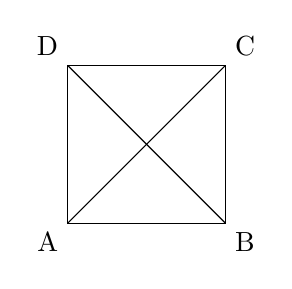
\begin{tikzpicture}[scale=1]
% Define vertices of the square
\coordinate (A) at (0,0);
\coordinate (B) at (2,0);
\coordinate (C) at (2,2);
\coordinate (D) at (0,2);
% Draw the square
\draw (A) -- (B) -- (C) -- (D) -- cycle;
% Draw the diagonals
\draw (A) -- (C);
\draw (B) -- (D);
% Label the vertices
\node[below left] at (A) {A};
\node[below right] at (B) {B};
\node[above right] at (C) {C};
\node[above left] at (D) {D};
\end{tikzpicture}
\end{center}
Se puede ver claramente que \textbf{A1} y \textbf{A2} se cumplen. Es trivial que \textbf{A3} se cumple.	
\end{eg}
\begin{theorem}
Si $\displaystyle \K $ es un cuerpo, entonces $\displaystyle \K^{2} $ es un plano afín con puntos $\displaystyle \K^{2} $ y rectas las ecuaciones lineales.
\end{theorem}
\begin{proof}
Adaptar la demostración del ejemplo del plano cartesiano.
\end{proof}
\begin{eg}
	Consideremos el cuerpo $\displaystyle \mathbb{F}_{2} = \left\{ 0,1\right\}  $ con la suma módulo 2 y el producto también módulo 2.
	Tenemos, por el teorema anterior, el plano afín $\displaystyle \mathbb{F}_{2}^{2} $ de la forma:
	\[\mathbb{F}_{2}^{2} = \left\{ \left(0,0\right), \left(1,0\right), \left(0,1\right), \left(1,1\right)\right\} .\]
	\[\mathcal{R} = \left\{ \left\{ x_{1} = 0\right\}, \left\{ x_{2} = 0\right\}, \left\{ x_{1} = 1\right\}, \left\{ x_{2} = 1\right\}, \left\{ x_{1} + x_{2} = 1\right\} \right\}  .\]
Gráficamente podemos ver que es igual al ejemplo anterior. En este caso, decimos que existe una colineación entre ellos.	
\end{eg}
\subsection{Independencia de los axiomas}
En primer lugar, estudiamos la independencia de \textbf{A3}. Consideremos un ejemplo que satisface \textbf{A1} y \textbf{A2}: $\displaystyle \mathcal{P} = \R $ y $\displaystyle \mathcal{R} = \left\{ l = \R\right\}  $. Así, tenemos que \textbf{A3} es independiente de los otros dos axiomas. \\ \\
Ahora vamos a ver la independencia de \textbf{A2} respecto de \textbf{A1} y \textbf{A3}. Para ello eplearemos el ejemplo del plano de Fano (Gino Fano, 1892):
\[\mathcal{P} = \left\{ A, B, C, D, E, F, G\right\}  .\]
\[\mathcal{R} = \left\{ \left\{ A, B, C\right\}, \left\{ C, D, E\right\}, \left\{ E, F, A\right\}, \left\{ A, G, D\right\}, \left\{ B, G, E\right\}, \left\{ C, G, F\right\} , \left\{ F, B, D\right\} \right\}  .\]
Tenemos que $\displaystyle \left|\mathcal{P}\right| = \left|\mathcal{R}\right| = 7 $. Está claro que se verifica \textbf{A3}, puesto que $\displaystyle \left|\mathcal{R}\right| = 7 $ y $\displaystyle \forall l \in \mathcal{R}, \left|l\right| = 3 $. 
Se puede ver gráficamente que se cumple \textbf{A1} y no se cumple \textbf{A2}, pues cualquier par de rectas se interseca y por tanto no existen rectas paralelas:
% Dibujo
Este es el plano proyectivo más pequeño. \\ \\
Ahora tenemos que estudiar la independencia de \textbf{A1} respecto de \textbf{A2} y \textbf{A3}. Consideremos
\[\mathcal{P}= \left\{ A, B, C, D\right\}  .\]
\[\mathcal{R} = \left\{ \left\{ A, B\right\} , \left\{ C, D\right\} \right\}  .\]
Tenemos que \textbf{A3} se verifica, pues $\displaystyle \left|\mathcal{R}\right| = 2 $ y $\displaystyle \left| \left\{ A,B\right\} \right| = \left| \left\{ C, D\right\} \right| = 2 $. Por otro lado, si $\displaystyle P \not\in \left\{ A,B\right\}  $, tenemos que $\displaystyle P \in \left\{ C,D\right\}  $, por lo que $\displaystyle \left\{ C,D\right\} | | \left\{ A,B\right\}  $. Lo mismo podemos decir si $\displaystyle P \not\in \left\{ C,D\right\}  $. Así, tenemos que se verifica \textbf{A2}. Sin embargo, no se cumple \textbf{A1} porque no existe ninguna recta que contenga a $\displaystyle A $ y $\displaystyle C $.
\subsection{Algunos teoremas}
\begin{lema}[Tricotomía]
Sea $\displaystyle \left(\mathcal{P}, \mathcal{R}\right) $ un plano afín. Sean $\displaystyle l, m \in \mathcal{R} $. Se cumple una y solo una de las siguientes afirmaciones:
\begin{enumerate}
\item $\displaystyle l = m $.
\item $\displaystyle l | | m $.
\item $\displaystyle l \cap m $ es un punto.
\end{enumerate}
\end{lema}
\begin{proof}
Si $\displaystyle l $ no es paralela a $\displaystyle m $, tenemos que $\displaystyle l \cap m \neq \emptyset $. Si $\displaystyle \left|l \cap m\right| = 1 $, tenemos que es un punto y se cumple \textbf{3}. Si $\displaystyle \left|l \cap m\right|\geq 2 $, tenemos que existen $\displaystyle P,Q \in l \cap m $. Por \textbf{A1}, dado que por dos puntos pasa una única recta, debe ser que $\displaystyle m = l $.
\end{proof}
\begin{theorem}[Rectas equipotentes]
Sea $\displaystyle \left(\mathcal{P}, \mathcal{R}\right) $ un plano afín. Todo par de rectas están en biyección.
\end{theorem}
\begin{proof}
Sean $\displaystyle l, m \in \mathcal{R} $.
\begin{description}
\item[Caso 1.] Si $\displaystyle l = m $, es trivial que $\displaystyle l $ y $\displaystyle m $ son equipotentes.
\item[Caso 2.] Supongamos $\displaystyle l \cap m = O $, donde $\displaystyle O \in \mathcal{P} $. Por \textbf{A3}, tenemos que existen $\displaystyle L \in l, M \in m $ tales que $\displaystyle M, L \neq O $. Por \textbf{A1}, existe una única $\displaystyle r \in \mathcal{R} $ tal que $\displaystyle L, M \in r $. Si $\displaystyle P \in l/ \left\{ L\right\}  $, tenemos que existe una única $\displaystyle r_{p} | | r $ tal que $\displaystyle P \in r_{p} $. 
\begin{center}
	\begin{tikzpicture}
% Coordinates
\coordinate (O) at (0,1);
\coordinate (L) at (-2,-1); % on l
\coordinate (M) at (2,-1);  % on m
\coordinate (P) at (-1,0); % between L and O on l

% Lines l and m through O
\draw[name path=l] (-2.5,-1.5) -- (0.5,1.5) node[right] {$l$};
\draw[name path=m] (2.5,-1.5) -- (-0.5,1.5) node[left] {$m$};

% Line r (horizontal) through L and M
\draw[name path=r] (L) -- (M) node[midway, above] {$r$};

% Dashed line through P parallel to r (horizontal)
%\draw[dashed] (P) -- ($(P)+(1,0)$);
%\draw[dashed] (P) -- ($(P)+(-1,0)$);
\draw[dashed] (-1.3,0) -- (1.3,0) node[above] {$r_p$};

% Points
\fill (O) circle (0.7pt) node[above] {$O$};
\fill (L) circle (0.7pt) node[left] {$L$};
\fill (M) circle (0.7pt) node[right] {$M$};
\fill (P) circle (0.7pt) node[left] {$P$};

% Axes for reference
\draw[->, thin] (-1.2,0) -- (1.2,0) node[right] {$x$};
\draw[->, thin] (0,-0.2) -- (0,2.5) node[above] {$y$};
\end{tikzpicture}
	\end{center}

	Podemos hacer un par de observaciones:
	\begin{description}
		\item[Observación 1.] Vamos a ver que $\displaystyle \forall P \in l/ \left\{ L\right\}  $ tenemos que $\displaystyle P \not\in r$, queremos ver que $\displaystyle r _{p} $ existe. Si $\displaystyle P \in l \cap r $, tenemos que $\displaystyle L, P \in l \cap r $, por lo que $\displaystyle l = r $, por lo que $\displaystyle M \in l $ y $\displaystyle O,M \in l  $ y $\displaystyle l = m $, que es una contradicción. Por tanto, podemos afirmar que $\displaystyle \forall P \in l $, $\displaystyle P \neq L $, $\displaystyle \exists r_{p} $ recta paralela a $\displaystyle r $ y $\displaystyle P \in r_{p} $.
		\item[Observación 2.] Tenemos que ver que $\displaystyle r_{p} \cap m $ es un punto. Si $\displaystyle r_{p} | | m $, como $\displaystyle r_{p} | | r $, $\displaystyle M \in m $ y $\displaystyle M \in r $, se tiene que $\displaystyle m = r $, por lo que $\displaystyle L \in r = m $ y $\displaystyle O \in m $, por lo que $\displaystyle m = l $, lo que es una contradicción. Por otro lado, si $\displaystyle r_{p} = m $, $\displaystyle P \in l $ y $\displaystyle P \in r_{p} = m $ y $\displaystyle O \in m,l $, por lo que $\displaystyle m = l $, que es una contradicción. Por tanto, debe ser que $\displaystyle r_{p}\cap m $ es un punto.
	\end{description}
	De esta manera, podemos definir la función
	\[
	\begin{split}
		f : l / \left\{ L\right\} & \to m / \left\{ M\right\} \\
		P & \to r_{p} \cap m.
	\end{split}
	\]
	Para ver que $\displaystyle f $ es biyectiva, vamos a ver que existe su inversa. En efecto, tenemos que $\displaystyle \forall Q \in m / \left\{ M\right\}  $, $\displaystyle Q \not\in r $ y $\displaystyle r_{Q}\cap l $ es un punto. Así, tenemos una función
	\[
	\begin{split}
		g : m/ \left\{ M\right\} & \to l / \left\{ L\right\} \\
		Q & \to r_{Q} \cap l.
	\end{split}
	\]
Para ver que $\displaystyle g = f^{-1} $ tenemos que ver que $\displaystyle g\circ f = id $ y que $\displaystyle f\circ g = id $:
\[
\begin{split}
	\left(g \circ f\right)\left(P\right) & = g\left(f\left(P\right)\right) = g\left(r_{p} \cap m\right) .
\end{split}
\]
Tenemos que $\displaystyle r_{f\left(P\right)} = r _{r_{p} \cap m} | | r $ y $\displaystyle r_{f\left(P\right)} $ pasa por $\displaystyle r_{p} \cap m $. Pero $\displaystyle r_{p} | | r $ y $\displaystyle r_{p} $ pasa por $\displaystyle r_{p} \cap m $. Por \textbf{A2}, tenemos que $\displaystyle r_{f\left(P\right)} = r_{p} $. Así, tenemos que
\[g\left(r_{p} \cap m\right) = r_{f\left(P\right)} \cap l = r_{p} \cap l = P .\]
\item[Caso 3.] Si $\displaystyle m | | l $ y $\displaystyle M \in m $, $\displaystyle L \in l $, tenemos que existe una recta $\displaystyle r $ tal que $\displaystyle M, L \in r $. Así, tenemos que $\displaystyle r \cap m $ y $\displaystyle r \cap l $ es un punto y por lo aplicado en el caso anterior, tenemos que existe una biyección entre $\displaystyle r $ y $\displaystyle m $ y entre $\displaystyle r $ y $\displaystyle l $.
	% Dibujo 3
\end{description}
\end{proof}

